%----------------------------------------------------------------------------
%\Aref{test}. fejezetben több valós hálózatot vizsgálok meg az addigra meghatározott saját policy-k segítségével, és megvizsgálom a keverék policy pontosságát, azaz azt, hogy mennyire térnének el a valós hálózatbeli utak a jelenlegitől akkor, ha az általam ismertetett policy-kel határoznánk meg azokat.
%----------------------------------------------------------------------------
\chapter{Repülési hálózat vizsgálata}\label{test}
%----------------------------------------------------------------------------

Ebben a fejezetben az \href{http://openflights.org/}{openflights.org} oldalon elérhető repülési adatbázis feldolgozását és ezen adatokon futtatott szimulációt mutatom be.

  %----------------------------------------------------------------------------
  \section{Az adatok}
  %----------------------------------------------------------------------------
  Az \href{http://openflights.org/}{openflights} lehetőséget biztosít különféle repülési adatok interaktív keresésére, regisztráció után pedig akár statisztikákat készíthetünk saját utazásainkról. Emellett elérhető a mindenkori aktuális, teljes adatbázisa is, amit többek között hivatalos forrásokból, illetve a felhasználóktól gyűjt.
  Az oldalon elérhető adatbázis világszerte mindenhonnan gyűjt és tárol reptéri, repülőtársasági és repülési út adatokat. Több, mint 9000 reptér, 19000 társaság és közel 60000 repülési út érhető el. Részletes adatok \aref{tab:table_repterek},~\aref{tab:table_repulesitarsasagok}, és a \aref{tab:table_repulesiutvonalak} táblázatokban.

    %----------------------------------------------------------------------------
    \subsection{Repterek}
    %----------------------------------------------------------------------------
    \begin{figure}[!ht]
      \centering
      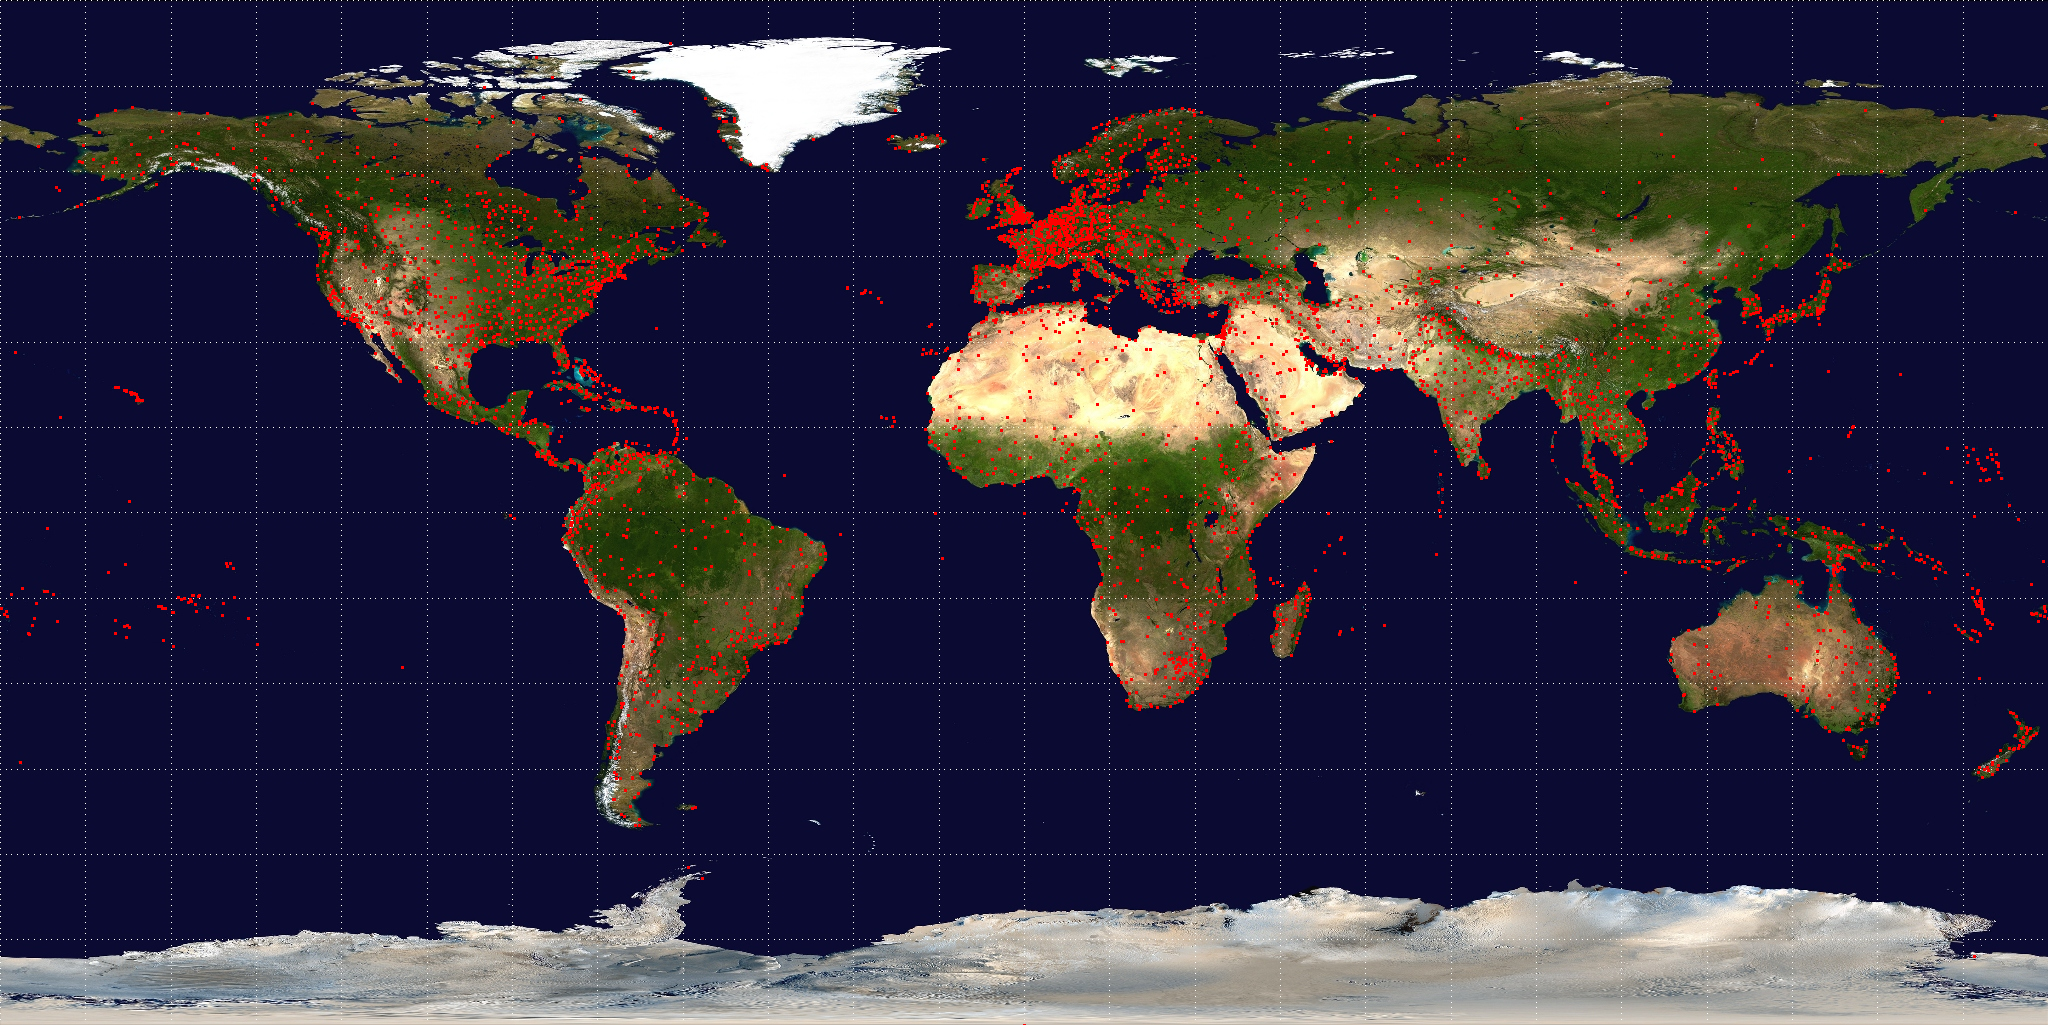
\includegraphics[width=150mm,keepaspectratio=true]{./figures/airports-2048.png}
      % airports-2048.png: 2048x1025 pixel, 96dpi, 54.18x27.12 cm

      \caption{Az OpenFights adatbázisában szereplő repterek.}
      \label{fig:figure_repterek}
    \end{figure}

    A rendszer tárolja a repterek \textit{nevét}; a \textit{várost}, ahol található; a \textit{szélességi}- és \textit{hosszúsági fokokat}, illetve a \textit{tengerszint feletti magasságot}. Emellett elérhető a repülési hatóságok által használt 3 karakter hosszú \textit{IATA\footnote{International Air Transport Association: Nemzetközi Légi Szállítási Szövetség}/FAA\footnote{Federal Aviation Administration: Szövetségi Légügyi Hivatal (USA)} azonosító} is és az OpenFlights által használt decimális \textit{azonosító} is. A legutolsó, 2014 januári frissítéskor az OpenFlights adatbázisa 9167 repteret tartalmazott világszerte, ezt mutatja \aref{fig:figure_repterek} ábra.

    \begin{table}[ht]
      \footnotesize
      \centering
      \caption{Az OpenFlights adatbázisában elérhető reptéri adatok.}
      \begin{tabular}{ | l | l |}
      \hline
      Attribútum & Leírás \\ \hline
      Airport ID & Egyedi OpenFlights azonosító.\\
      Name & A reptér neve.\\
      City & Az a város, amit a reptér ,,kiszolgál''.\\
      Country & Az ország vagy terület neve, ahol reptér található.\\
      IATA/FAA & 3 betűs FAA kód az USA-beli reptereknek vagy 3 betűs IATA kód, minden más esetben.\\
      ICAO\footnote{International Civil Aviation Organization: Nemzetközi Polgári Repülési Szervezet} & 4 betűs ICAO kód.\\
      Latitude & A reptér szélességi foka: decimális szám (fokban mérve), általában 6 szignifikáns jegyig.\\
      & A Déli féltekén negatív, az Északin pozitív.\\
      Longitude & A reptér hosszúsági foka: decimális szám (fokban mérve), általában 6 szignifikáns jegyig.\\
      & A Nyugati féltekén negatív, a Keletin pozitív.\\
      Altitude & A tengerszint feletti magasság, lábban mérve (1 láb $\sim$ 0.30 méter).\\
      \hline
      \end{tabular}
      \label{tab:table_repterek}
    \end{table}

    %----------------------------------------------------------------------------
    \subsection{Repülési útvonalak}
    %----------------------------------------------------------------------------
    \begin{figure}[!ht]
      \centering
      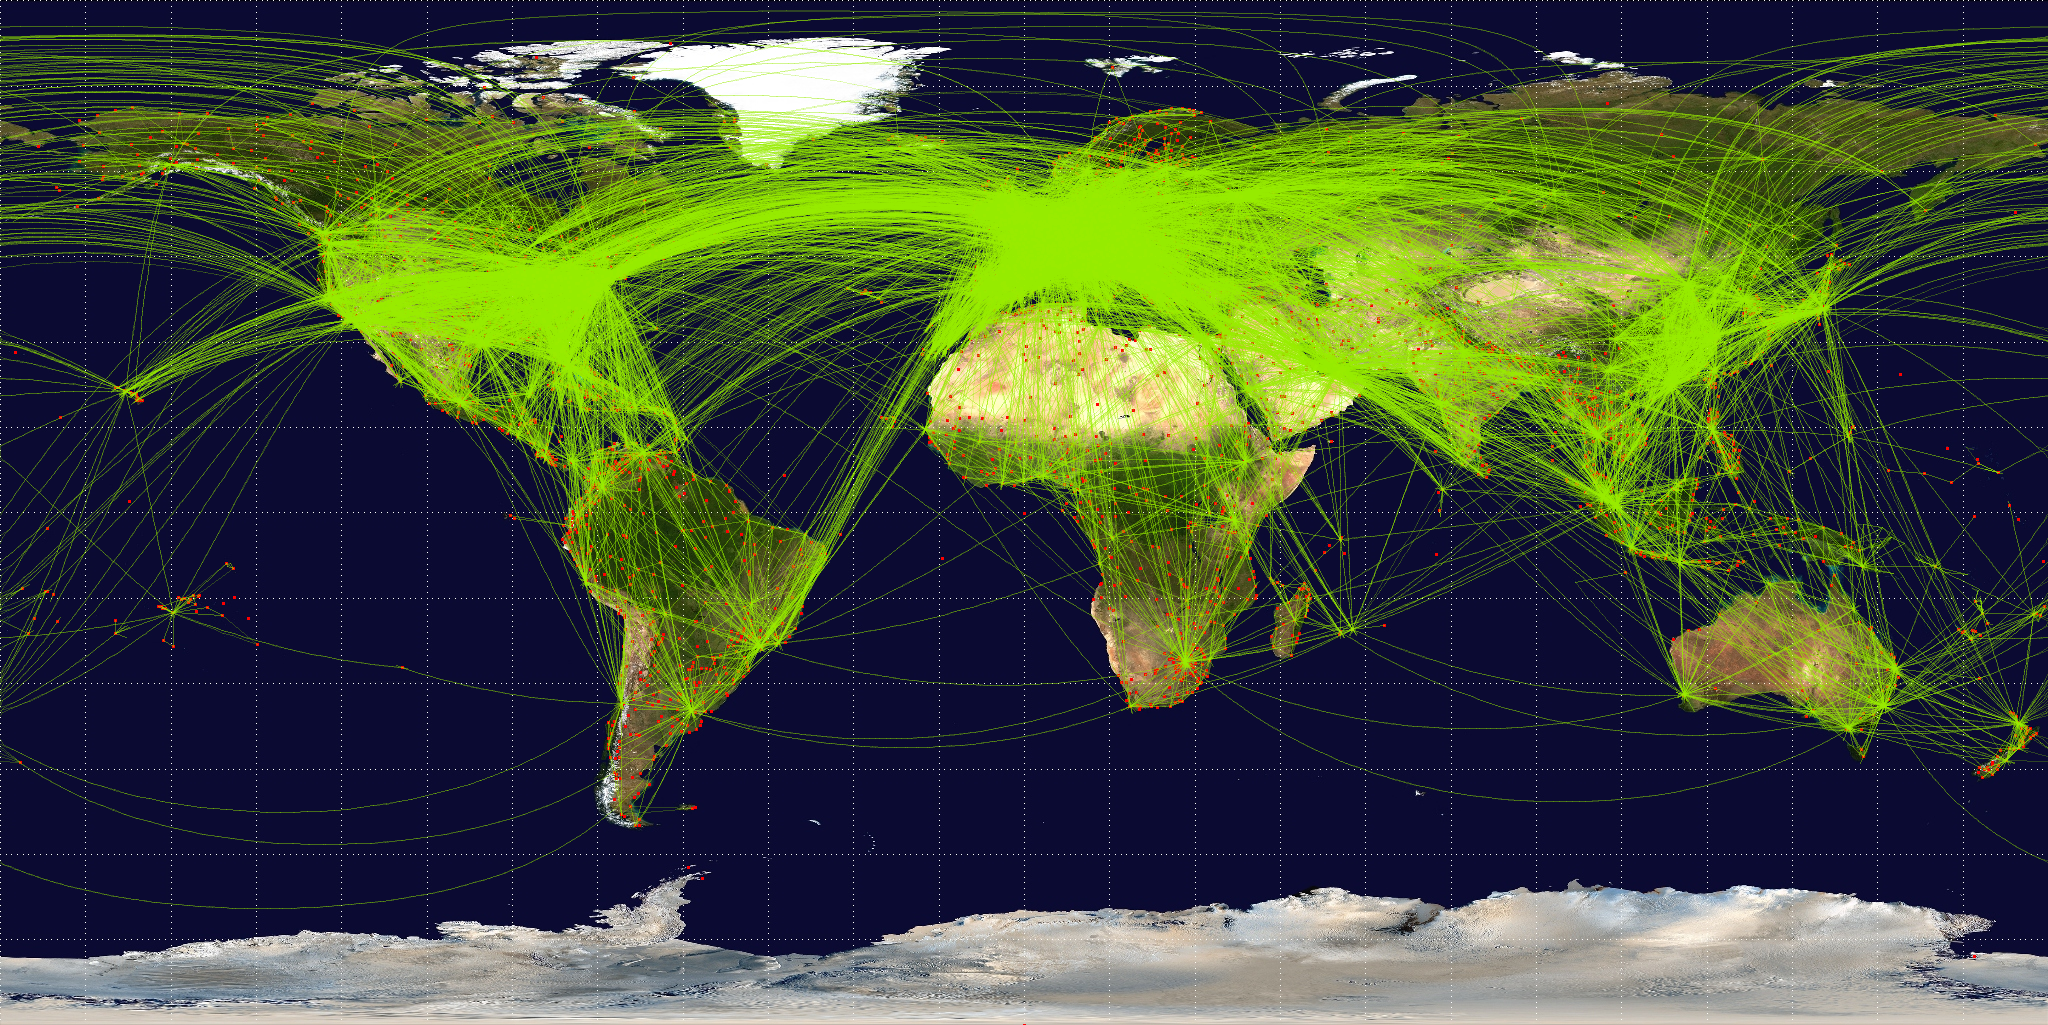
\includegraphics[width=150mm,keepaspectratio=true]{./figures/routes-2048.png}
      % routes-2048.png: 2048x1025 pixel, 96dpi, 54.18x27.12 cm

      \caption{Az OpenFights adatbázisában szereplő repülési útvonalak.}
      \label{fig:figure_repulesiutvonalak}
    \end{figure}

    A repülési útvonalak leírása öt attribútumot tartalmaz: az \textit{üzemeltető repülőtársaság} (név és OpenFlights azonosító); a \textit{forrás reptér}; a \textit{cél reptér}. Emellett feljegyzik a \textit{megállások számát}\footnote{Az összesen 59637 bejegyzésből 6 esetében van 1 megállás és 1 esetben 2 megállás, ezért ezt az adatot a szimuláció során semmilyen módon nem használom fel.}, illetve az ebben a viszonylatban használt \textit{repülőgép típusokat}. Ha két reptér között oda-vissza is van járat, akkor ez az adathalmazban két bejegyzésként jelenik meg. Jelenleg az OpenFlights adatbázisa 59637 útvonalat tartalmazott 3285 reptér és 531 társaság\footnote{Ugyan a légitársaság és reptér adatbázisokban ennél jelentősen több bejegyzés van, ám azok között vannak nem aktív társaságok, illetve bezárt repterek.} között világszerte, ahogy \aref{fig:figure_repulesiutvonalak} ábra is mutatja.

    \begin{table}[ht]
      \footnotesize
      \centering
      \caption{Az OpenFlights adatbázisában elérhető adatok a repülési útvonalakról.}
      \begin{tabular}{ | l | l |}
      \hline
      Attribútum & Leírás \\ \hline
      Airline & Az üzemeltető társaság 2 betűs (IATA) vagy 3 betűs (ICAO) kódja.\\
      Airline ID & Az üzemeltető társaság egyedi OpenFlights azonosítója.\\
      Source airport & A forrás reptér 3 betűs (IATA) vagy 4 betűs (ICAO) kódja.\\
      Source airport ID & A forrás reptér egyedi OpenFlights azonosítója.\\
      Destination airport & A cél reptér 3 betűs (IATA) vagy 4 betűs (ICAO) kódja.\\
      Destination airport ID & A cél reptér egyedi OpenFlights azonosítója.\\
      Codeshare & Igaz, ha a járat ,,codeshare'', azaz nem utasszállító járat, különben üres.\\
      Stops & A megállások szám (nem az átszállásokat jelenti, a ,,0'' jelenti a direkt járatot).\\
      Equipment & A viszonylatban használt repülőgép típusok 3 betűs kódjai.\\
      \hline
      \end{tabular}
      \label{tab:table_repulesiutvonalak}
    \end{table}

    %----------------------------------------------------------------------------
    \subsection{Repülőtársaságok}
    %----------------------------------------------------------------------------
    A repülőtársaságokról tárolt adatok többek között tartalmazzák a hivatalos \textit{IATA azonosítót}; a cég \textit{nevét}; az \textit{országot}, ahol be van jegyezve; illetve, hogy \textit{aktív-e} még a társaság. Emellett természetesen itt is definiáltak egy saját (OpenFlights) \textit{azonosítót}.

    \begin{table}[ht]
      \footnotesize
      \centering
      \caption{Az OpenFlights adatbázisában elérhető adatok a repülőtársaságokról.}
      \begin{tabular}{ | l | l |}
      \hline
      Attribútum & Leírás \\ \hline
      Airport ID & Egyedi OpenFlights azonosító.\\
      Name & A társaság neve.\\
      Alias & A társaság egyéb megnevezése.\\
      IATA & 2 betűs IATA kód.\\
      ICAO & 3 betűs ICAO kód.\\
      Callsign & A társaság hívójele.\\
      Country & Az ország vagy terület neve, ahol a társaság be van jegyezve.\\
      Active & Igaz, ha a társaság jelenleg is, vagy nemrég még működött (nem megbízható).\\
      \hline
      \end{tabular}
      \label{tab:table_repulesitarsasagok}
    \end{table}

  %----------------------------------------------------------------------------
  \section{A szimuláció}
  %----------------------------------------------------------------------------
  \Aref{framework} fejezetben ismertetett keretrendszert használva fogom megvizsgálni a fent bemutatott adathalmazon a $\mathcal{S}$ (Shortest algebra), a $\mathcal{L}$ (LeastHop algebra: $\mathcal{L}$ = ($\mathbb{N},~\infty,~+,~\leq$), legkevesebb csomópontot érintő út), az $\mathcal{O}$ (Összekötő-keresés: \ref{osszekoto_kereses}. rész) és a $\mathcal{K}$ (Korai-elfogadó-keresés: \ref{korai_elfogado_kereses}. rész) algebrákat. Mivel az utolsó kettő algebra nem jól viselkedő\footnote{Világos, hogy $\geq$ operátorú algebrák maximumot keresnek, ami ezeknél a konkrét algebráknál maximális utak keresését jelenti. Viszont \aref{max_route}. tétel értelmében csak akkor tudunk maximális utakat keresni, ha a gráf DAG, ami nyilvánvalóan ebben az esetben nem áll fenn, hiszen ez azt jelentené, hogy egy reptérről indul soha nem juthatunk vissza ugyanoda.}, ezért csak a $\mathcal{S}$, $\mathcal{L}$, $\mathcal{OS}$, $\mathcal{KS}$, $\mathcal{OL}$ és a $\mathcal{KL}$ algebrákat fogom ténylegesen szimulálni, mert a lexikografikus szorzatban már csak egy adott útvonalhalmazból kell kiválasztani a szorzat első tényezője szerinti legjobbat.

    %----------------------------------------------------------------------------
    \subsection{Az adatok előfeldolgozása}
    %----------------------------------------------------------------------------
    A modellezendő hálózat első megközelítésben az összes csomópontból alkotott $K_{9167}$ teljes gráf. Ez természetesen feleslegesen nagy hálózatot jelent ($9167 \choose 2$ = 42 012 361 élű gráf.), emellett az olyan, leíró jellegű jellemzők, mint a valódi hálózat átmérője, vagy az élösszefüggőség elvesznének. Lévén a repülési hálózat skálafüggetlen - sok olyan csomópont van, ahova csak adott, kis számú, közeli csomópontokból indulnak járatok, így nem érdemes összekötni távoli csomópontokkal. Ezenkívül a repülésnél vannak olyan szempontok, amelyeket az útvonalválasztásnál figyelembe vesznek, ám én ezek pontos információk hiányában nem tudom kezelni - pl. csak adott hosszúságú utat tehet meg egy adott típusú repülőgép az üzemanyagtartálya méretétől függően.\\

    A fentiek miatt a szimulált hálózatot a következőképpen határozom meg: pontjai a repterek, élei pedig, az adatbázisban szereplő össze, megállás nélküli repülőút. Így magától értetődően csak olyan élek lesznek a szimulációban, amelyek ,,átrepülhetők'', hiszen volt már, hogy átrepülték. Emellett pedig ez a hálózat hűen tükrözi a valóságot, hiszen feltehetjük, hogy csak azon élek nincsenek behúzva, amelyeket repüléstechnikai okokból nem is lehet, különben valaki, valamikor már repült volna azon az úton.

      %----------------------------------------------------------------------------
      \subsubsection{Az élsúlyok meghatározása}
      %----------------------------------------------------------------------------
      Ahogy \aref{prep}. részben kifejtettem, a vizsgálni kívánt algebráktól függően határozom meg az élsúlyozást, valamint a súlyozás során az eredményt nem jelentősen befolyásoló és a futást gyorsító egyszerűsítésekkel élhetek.\\

      A $\mathcal{S}$ algebra miatt szükséges a csomópontok valós távolságára. Ezt a repterek szélességi és hosszúsági koordinátái alapján a Haversine formulával számolom. Annak érdekében, hogy pontos, de mégsem túl nagy számokat kapjak a távolságot [km]-ben mért egész számmal jelölöm (az akár [m]-ben mért egytizedes pontosság helyett).\\
      A $\mathcal{L}$ algebra pusztán az élek létét használja fel, így minden él súlya 1.\\
      Az $\mathcal{O}$ algebra a népszerű reptereket részesíti előnyben, ami azt jelenti, hogy itt egy csúcs érték $\rightarrow$ élsúly konverzióra van szükség. Mivel a gráf irányított, nem kell azzal törődni, hogy egy esetleges hibás megadás esetén az él súlyát akkor is terheli a népszerű reptér, amikor onnan elfelé haladunk. Egyszerűen minden csomópontra, a befelé mutató éleket a csomópont népszerűsége szerint súlyozunk. Ez a tényleges megvalósítást tekintve azt jelenti, hogy a repterekre érkező és az onnan induló járatok, tehát a reptér teljes forgalma adja meg a csomópont népszerűségét.\\
      A $\mathcal{K}$ algebra esetén azon az úton fogunk haladni, amin a legtöbben haladtak, így minden élnek a súlyát úgy határozzuk meg, hogy a megfigyelések szerint hányszor repültek az adott viszonylaton.

    %----------------------------------------------------------------------------
    \subsection{A szimuláció menete}
    %----------------------------------------------------------------------------
    A repülési adatok ismeretében nem pontosan \aref{section_simulator}. részben ismertetett módon szimulálok. A gráf élhalmaza a repülési adatokból kapott utak, és ezen a gráfon a 10 legjelentősebb légitársaság útvonalait vizsgálom meg. Bár az előző fejezetben ismertetett szimulátor minden pontpárra előírná az útvonal meghatározását, de jelen esetben a skálafüggetlenség miatt a szimulált utak túlnyomó többsége - a fokszámeloszlás szerinti ,,farkok'' csúcsai kis fokszámúak - nem is lehet más, mint a megfigyelt út. Ez eltorzítaná a szimulációt, hiszen magas pontot ér, ha pontos a becslés. Ezzel szemben, ha csak a 10 legtöbb járatot üzemeltető társaságot veszem figyelembe, akkor \aref{elossze}. részben leírt \textit{mag}hoz hasonlóan a lényeget kiemelve tudom vizsgálni a problémát: a 10 legtöbb járatot indító társaság bonyolítja le a repülőutak 24\%-át.
    % 5209 (2417), 4296 (2186), 2009 (1520), 24 (1513), 5265 (1381), 751 (1227), 1767 (1152), 1758 (1097), 4547 (1018), 3320 (931),

  %----------------------------------------------------------------------------
  \section{Az eredmények}
  %----------------------------------------------------------------------------

        \todo

  %----------------------------------------------------------------------------
  \section{Összefoglaló}
  %----------------------------------------------------------------------------
  Ebben a fejezetben \aref{framework}. fejezetben leírt keretrendszert használva megvizsgáltam egy valós hálózatot az \href{http://openflights.org/}{openflights} repülési adatbázisát felhasználva. A szimulációs keretrendszerben meghatározott lépéseket elvégeztem, a szükséges módosításokat megtettem, ahol a probléma miatt erre muszáj volt. A repülési adatbázis alapján létrehoztam az irányított, vektor-súlyozott gráfot, az élsúlyokat a vizsgálandó algebrák alapján számítottam ki és rendeltem az élekhez.\\

  A kész tervet a saját magam írt szimulátor szoftverrel hajtottam végre, az eredményeket közönséges táblázatkezelővel elemeztem ki. Megvizsgáltam a Shortest ($\mathcal{S}$), a LeastHop ($\mathcal{L}$), az Összekötő-keresés ($\mathcal{O}$) és a Korai-elfogadó-keresés ($\mathcal{K}$) algebrákat, illetve az Összekötő-keresés-Shortest ($\mathcal{OS}$), a Korai-elfogadó-keresés-Shortest ($\mathcal{KS}$), az Összekötő-keresés-LeastHop ($\mathcal{OL}$) és a Korai-elfogadó-keresés-LeastHop ($\mathcal{KL}$) lexikografikus szorzatként előálló összetett algebrákat is.